\section{Schematy różnicowe dla zadań dyfuzyjnych}

Będziemy korzystać z równania:

\[
\begin{cases}
\vspace{0.1cm} 
\hspace{0,1cm} \dfrac{\delta \psi}{\delta t} = D\dfrac{\delta^2 \psi}{\delta x^2} \hspace{1cm}, \Omega = [0,L]x[0,\infty] \\
\vspace{0.1cm}
\hspace{0,1cm}\psi_{(x,t)}|_{x=0} = 0 \hspace{0.8cm},t>0 \\
\vspace{0.1cm} 
\hspace{0,1cm}\psi_{(x,t)}|_{x=L} = 0 \hspace{0.7cm},t>0 \\
\vspace{0.1cm} 
\hspace{0,1cm}\psi_{(x,t)}|_{t=0} = \varphi(x) \hspace{0.3cm},x\in[0,L]
\end{cases}
\]

Przyjmujemy następującą konwencję oznaczeń:

\fontsize{14}{2}

$$\psi_{(x_i,t_n)} = \psi^{n}_{i}$$

\fontsize{11}{1}

, gdzie:

n - czas

i - przestrzeń

\subsection{Cel ćwiczenia}

Naszym zadaniem było stworzenie algorytmu rozwiązującego następujące równanie:

\[
\begin{cases}
\vspace{0.1cm} 
\hspace{0,1cm} \dfrac{\delta \psi}{\delta t} = D\dfrac{\delta^2 \psi}{\delta x^2} \\
\vspace{0.1cm}
\hspace{0,1cm}\psi|_{x=0} = 0 \\
\vspace{0.1cm} 
\hspace{0,1cm}\psi|_{x=L} = 0 \\
\vspace{0.1cm} 
\hspace{0,1cm}\psi|_{t=0} = sin(\frac{\pi x}{2})
\end{cases}
\]

, gdzie:

$\Omega = [0,2]x[0,1]$
\newline
$D=1$
\newline
\vspace{0.2cm}
$\psi_{analityczna}=\psi(x,t)=sin\Big(\dfrac{\pi x}{2}\Big)e^{-\Big(\dfrac{\pi^2 t}{4}\Big)}$

\subsection{Schemat FTCS}

FTCS (ang. Forward Time Central Space) czyli schemat "w przód":

$$\dfrac{\delta \psi}{\delta t} = D\dfrac{\delta^2 \psi}{\delta x^2}$$

Dla lewej strony równania zastosujemy schemat "w przód", natomiast dla prawej schemat centralny.

Mamy więc:

$$\dfrac{\psi^{(n+1)}_{i}-\psi^n_{i}}{\Delta t}=D\dfrac{\psi^{n}_{i+1}-2\psi^n_{i}+\psi^n_{i-1}}{\Delta x^2}$$

Stąd:

$$\psi^{(n+1)}_{i}=\dfrac{D\Delta t}{\Delta x^2}\Big(\psi^{n}_{i+1}-2\psi^{n}_{i}+\psi^{n}_{i-1}\Big)+\psi^{n}_{i} + O(\Delta t)+O(\Delta x^2)$$

Jest to schemat jawny, warunkowo stabilny, a więc parametry siatki muszą zostać dobrane we właściwy sposób.

Warunkiem stabilności dla takiego zadania jest następująca relcja:

$$\dfrac{D\Delta t}{\Delta x^2}\le \dfrac{1}{2}$$

\subsubsection{Algorytm}

\begin{Shaded}
\begin{Highlighting}[]
\FunctionTok{clc}\NormalTok{,}\FunctionTok{clear} \FunctionTok{all}
\FunctionTok{tic}
\CommentTok{%rozwiązanie analityczne}
\NormalTok{G = @(x,t) }\FunctionTok{sin}\NormalTok{(}\BaseNTok{pi}\NormalTok{.*x./}\FloatTok{2}\NormalTok{).*}\FunctionTok{exp}\NormalTok{(-(}\BaseNTok{pi}\NormalTok{.^}\FloatTok{2}\NormalTok{).*t./}\FloatTok{4}\NormalTok{);}

\CommentTok{%przedział omega}
\NormalTok{xa=}\FloatTok{0}\NormalTok{;}
\NormalTok{xb=}\FloatTok{2}\NormalTok{;}
\NormalTok{yc=}\FloatTok{0}\NormalTok{;}
\NormalTok{yd=}\FloatTok{1}\NormalTok{;}

\CommentTok{%warunki brzegowe}
\NormalTok{u1 = @(x) }\FloatTok{0}\NormalTok{;}
\NormalTok{u2 = @(x) }\FloatTok{0}\NormalTok{;}
\NormalTok{u3 = @(x,t) }\FunctionTok{sin}\NormalTok{(}\BaseNTok{pi}\NormalTok{*x/}\FloatTok{2}\NormalTok{);}

\NormalTok{licznik=}\FloatTok{0}\NormalTok{;}
\CommentTok{%siatka}
\NormalTok{m=}\FloatTok{30}\NormalTok{;}
\NormalTok{D=}\FloatTok{1}\NormalTok{;}
\NormalTok{deltax=(xb-xa)/(m-}\FloatTok{1}\NormalTok{);}
\NormalTok{x=[xa:deltax:xb];         }\CommentTok{%przedział przestrzenny}
\NormalTok{deltat=(deltax^}\FloatTok{2}\NormalTok{)/(}\FloatTok{20}\NormalTok{*D); }\CommentTok{%dzielimy od razu przez 10, aby wartość }
\NormalTok{n_end=}\FunctionTok{floor}\NormalTok{(yd/deltat)+}\FloatTok{1}\NormalTok{; }\CommentTok{%nie była blisko deltat graniczne}
\NormalTok{t=[}\FloatTok{0}\NormalTok{:deltat:}\FloatTok{1}\NormalTok{];           }\CommentTok{%przedział czasowy}

\CommentTok{%macierz}
\FunctionTok{psi}\NormalTok{=}\FunctionTok{zeros}\NormalTok{(n_end,}\FunctionTok{length}\NormalTok{(x)); }\CommentTok{%utworzenie pustej macierzy}

\NormalTok{for }\BaseNTok{i}\NormalTok{=}\FloatTok{2}\NormalTok{:m-}\FloatTok{1}                \CommentTok{%dodanie warunku początkowego}
  \FunctionTok{psi}\NormalTok{(}\FloatTok{1}\NormalTok{,}\BaseNTok{i}\NormalTok{)=u3(x(}\BaseNTok{i}\NormalTok{));}
\NormalTok{end}
                        
\NormalTok{for n=}\FloatTok{2}\NormalTok{:n_end}
\NormalTok{  for }\BaseNTok{i}\NormalTok{=}\FloatTok{2}\NormalTok{:m-}\FloatTok{1}
    \FunctionTok{psi}\NormalTok{(n,}\BaseNTok{i}\NormalTok{)=(deltat/deltax^}\FloatTok{2}\NormalTok{)*(}\FunctionTok{psi}\NormalTok{(n-}\FloatTok{1}\NormalTok{,}\BaseNTok{i}\NormalTok{+}\FloatTok{1}\NormalTok{)-}\FloatTok{2}\NormalTok{*}\FunctionTok{psi}\NormalTok{(n-}\FloatTok{1}\NormalTok{,}\BaseNTok{i}\NormalTok{)+}\FunctionTok{psi}\NormalTok{(n-}\FloatTok{1}\NormalTok{,}\BaseNTok{i}\NormalTok{-}\FloatTok{1}\NormalTok{))+}\FunctionTok{psi}\NormalTok{(n-}\FloatTok{1}\NormalTok{,}\BaseNTok{i}\NormalTok{);}
\NormalTok{  end}
\NormalTok{  licznik = licznik+}\FloatTok{1}\NormalTok{;}
\NormalTok{end}

\NormalTok{[X,T] = }\FunctionTok{meshgrid}\NormalTok{(x,t);}
\FunctionTok{subplot}\NormalTok{(}\FloatTok{1}\NormalTok{,}\FloatTok{2}\NormalTok{,}\FloatTok{1}\NormalTok{)}
\FunctionTok{surf}\NormalTok{(X,T,}\FunctionTok{psi}\NormalTok{)}
\FunctionTok{title}\NormalTok{(}\StringTok{'Metoda Numeryczna'}\NormalTok{)}
\FunctionTok{subplot}\NormalTok{(}\FloatTok{1}\NormalTok{,}\FloatTok{2}\NormalTok{,}\FloatTok{2}\NormalTok{)}
\FunctionTok{surf}\NormalTok{(X,T,(G(X,T)))}
\FunctionTok{title}\NormalTok{(}\StringTok{'Metoda Analityczna'}\NormalTok{)}
\NormalTok{licznik}
\FunctionTok{toc}
\end{Highlighting}
\end{Shaded}
\newpage
\subsubsection{Wykresy}

Dla n = 5:

\begin{figure}[!ht]
	\begin{center}
		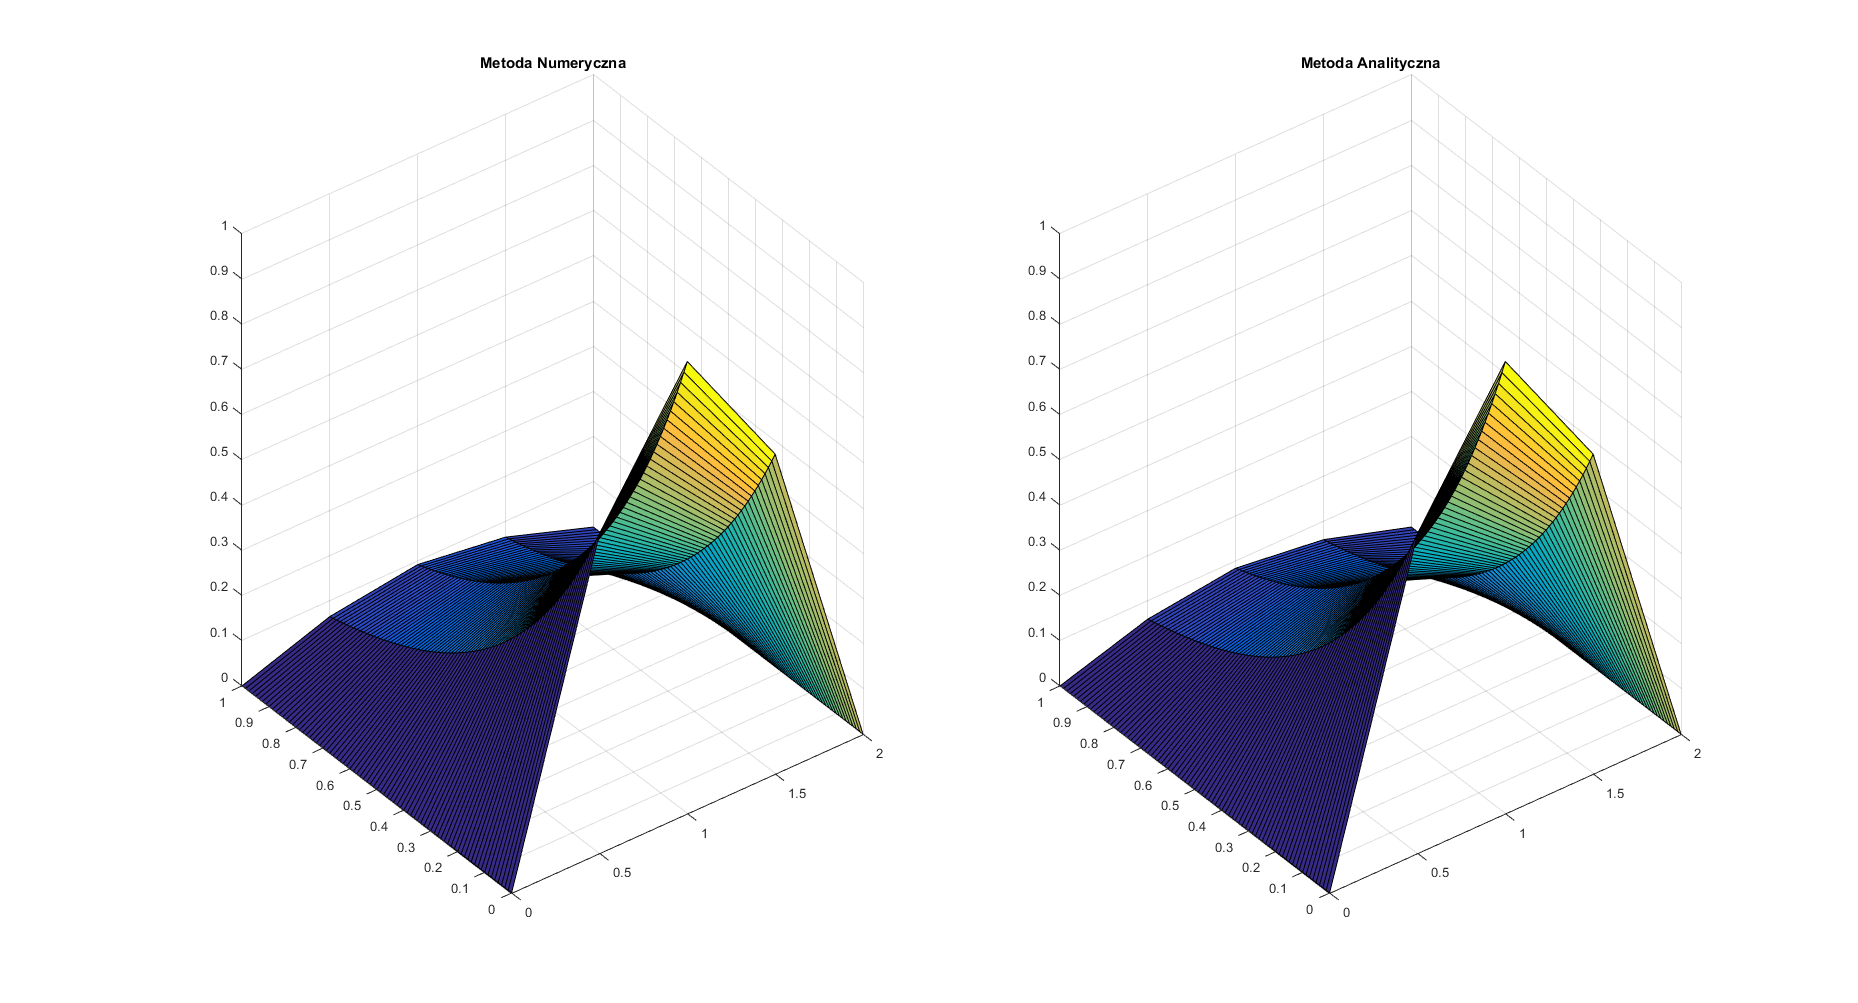
\includegraphics[width=0.78\textwidth]{Lab7/charts/ftcs/5.png}
	\end{center}
\end{figure}

Czas wykonywania algorytmu $ = 0.102 s$

Dla n = 15:

\begin{figure}[!ht]
	\begin{center}
		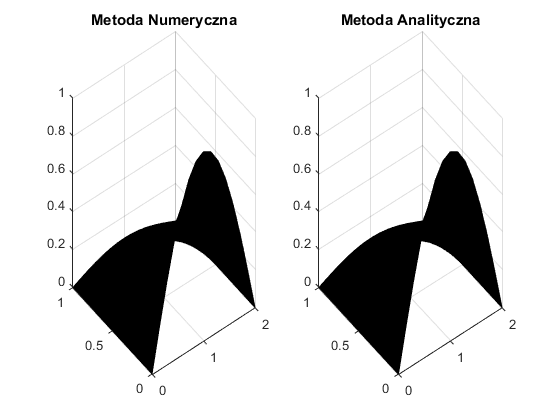
\includegraphics[width=0.78\textwidth]{Lab7/charts/ftcs/15.png}
	\end{center}
\end{figure}

Czas wykonywania algorytmu $ = 0.163 s$

\newpage

Dla n = 30:

\begin{figure}[!ht]
	\begin{center}
		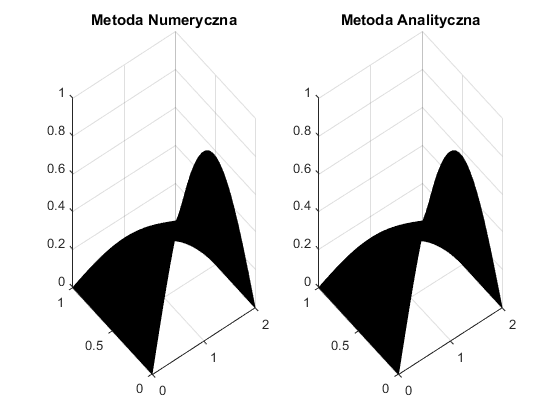
\includegraphics[width=0.78\textwidth]{Lab7/charts/ftcs/30.png}
	\end{center}
\end{figure}

Czas wykonywania algorytmu $ = 0.472 s$

Jeżeli warunek stabilności nie zostanie spełniony:

Dla:

$$\dfrac{D\Delta t}{\Delta x^2} = \dfrac{1}{2}$$

\begin{figure}[!ht]
	\begin{center}
		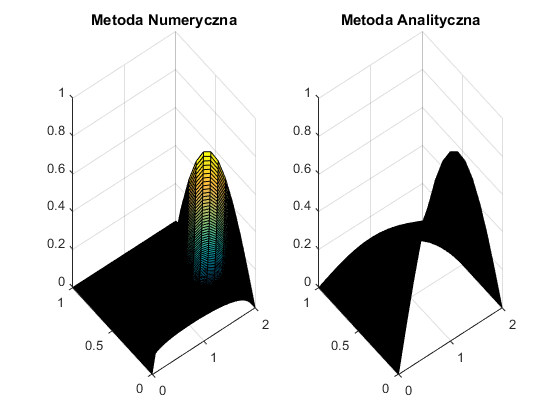
\includegraphics[width=0.78\textwidth]{Lab7/charts/ftcs/oscylowanko05.png}
	\end{center}
\end{figure}

\newpage

Dla:

$$\dfrac{D\Delta t}{\Delta x^2} = \dfrac{6}{10}$$

\begin{figure}[!ht]
	\begin{center}
		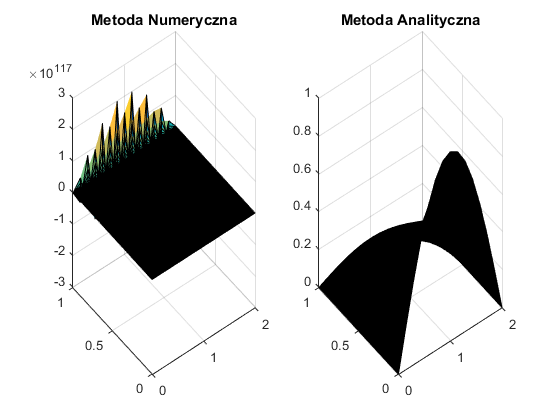
\includegraphics[width=0.78\textwidth]{Lab7/charts/ftcs/oscylowanko06.png}
	\end{center}
\end{figure}

\subsection{Schemat BTCS}
BTCS (ang. Backward Time Central Space) czyli schemat "w tył":

$$\dfrac{\delta \psi}{\delta t} = D\dfrac{\delta^2 \psi}{\delta x^2}$$

Dla lewej strony równania zastosujemy schemat "w tył", natomiast dla prawej schemat centralny.

Mamy więc:

$$\dfrac{\psi^{(n+1)}_{i}-\psi^n_{i}}{\Delta t}=D\dfrac{\psi^{n}_{i+1}-2\psi^n_{i}+\psi^n_{i-1}}{\Delta x^2} + O(\Delta t)+O(\Delta x^2)$$

Stąd:

$$-\psi^{(n+1)}_{i+1} + \left(2+\dfrac{\Delta x^2}{D \Delta t}\right) \psi^{(n+1)}_{i} -\psi^{(n+1)}_{i-1} =\dfrac{\Delta x^2}{D\Delta t}\psi^{n}_{i}$$

Jest to schemat jawny, bezwzględnie stabilny. 

Z powyższego równania otrzymujemy liniowy układ równań algebraicznych, a więc w każdej iteracji czasowej należy rozwiązać pewien układ równań liniowych.
\newpage
\subsubsection{Algorytm}
\begin{Shaded}
\begin{Highlighting}[]
\FunctionTok{clc}\NormalTok{,}\FunctionTok{clear} \FunctionTok{all}\NormalTok{; }\FunctionTok{tic}
\CommentTok{%rozwiązanie analityczne}
\NormalTok{G = @(x,t) }\FunctionTok{sin}\NormalTok{(}\BaseNTok{pi}\NormalTok{.*x./}\FloatTok{2}\NormalTok{).*}\FunctionTok{exp}\NormalTok{(-(}\BaseNTok{pi}\NormalTok{.^}\FloatTok{2}\NormalTok{).*t./}\FloatTok{4}\NormalTok{);}
\CommentTok{%przedział omega}
\NormalTok{xa=}\FloatTok{0}\NormalTok{; xb=}\FloatTok{2}\NormalTok{; yc=}\FloatTok{0}\NormalTok{; yd=}\FloatTok{1}\NormalTok{;}
\CommentTok{%warunki brzegowe}
\NormalTok{u1 = @(x) }\FloatTok{0}\NormalTok{;}
\NormalTok{u2 = @(x) }\FloatTok{0}\NormalTok{;}
\NormalTok{u3 = @(x,t) }\FunctionTok{sin}\NormalTok{(}\BaseNTok{pi}\NormalTok{*x/}\FloatTok{2}\NormalTok{);}
\NormalTok{licznik=}\FloatTok{0}\NormalTok{;}
\CommentTok{%siatka}
\NormalTok{m=}\FloatTok{20}\NormalTok{; D=}\FloatTok{1}\NormalTok{;}
\NormalTok{deltax=(xb-xa)/(m-}\FloatTok{1}\NormalTok{);}
\NormalTok{x=[xa:deltax:xb];         }\CommentTok{%przedział przestrzenny}
\NormalTok{deltat=(deltax^}\FloatTok{2}\NormalTok{)/(}\FloatTok{10}\NormalTok{*D); }
\NormalTok{n_end=}\FunctionTok{floor}\NormalTok{(yd/deltat)+}\FloatTok{1}\NormalTok{; }
\NormalTok{t=[}\FloatTok{0}\NormalTok{:deltat:}\FloatTok{1}\NormalTok{];           }\CommentTok{%przedział czasowy}
\CommentTok{%macierz}
\FunctionTok{psi}\NormalTok{=}\FunctionTok{zeros}\NormalTok{(n_end,}\FunctionTok{length}\NormalTok{(x)); }\CommentTok{%utworzenie pustej macierzy}
\CommentTok{%dodanie warunku początkowego}
\FunctionTok{psi}\NormalTok{(}\FloatTok{1}\NormalTok{,:) = u3(x);}
\FunctionTok{psi}\NormalTok{(:,}\FloatTok{1}\NormalTok{) = u1(t);}
\FunctionTok{psi}\NormalTok{(:,m) = u2(t);}
\NormalTok{A = (}\FloatTok{2}\NormalTok{+(deltax^}\FloatTok{2}\NormalTok{)/(deltat))*}\FunctionTok{diag}\NormalTok{(}\FunctionTok{eye}\NormalTok{(m-}\FloatTok{2}\NormalTok{));}
\NormalTok{B = }\FunctionTok{diag}\NormalTok{(A) + -}\FloatTok{1}\NormalTok{*}\FunctionTok{diag}\NormalTok{(}\FunctionTok{diag}\NormalTok{(}\FunctionTok{eye}\NormalTok{(m-}\FloatTok{3}\NormalTok{)),-}\FloatTok{1}\NormalTok{) + -}\FloatTok{1}\NormalTok{*}\FunctionTok{diag}\NormalTok{(}\FunctionTok{diag}\NormalTok{(}\FunctionTok{eye}\NormalTok{(m-}\FloatTok{3}\NormalTok{)),}\FloatTok{1}\NormalTok{);}
\NormalTok{for n=}\FloatTok{2}\NormalTok{:n_end}
\NormalTok{  F = }\FunctionTok{diag}\NormalTok{(}\FunctionTok{eye}\NormalTok{(m-}\FloatTok{2}\NormalTok{)) * deltax^}\FloatTok{2}\NormalTok{/deltat .* }\FunctionTok{psi}\NormalTok{(n-}\FloatTok{1}\NormalTok{,}\FloatTok{2}\NormalTok{:m-}\FloatTok{1}\NormalTok{)';}
\NormalTok{  F(}\FloatTok{1}\NormalTok{) = F(}\FloatTok{1}\NormalTok{) + }\FunctionTok{psi}\NormalTok{(n,}\FloatTok{1}\NormalTok{);}
\NormalTok{  F(}\FunctionTok{length}\NormalTok{(F)) = F(}\FunctionTok{length}\NormalTok{(F)) + }\FunctionTok{psi}\NormalTok{(n, m);  }
  \FunctionTok{psi}\NormalTok{(n,}\FloatTok{2}\NormalTok{:m-}\FloatTok{1}\NormalTok{) = linsolve(B,F);}
\NormalTok{  licznik = licznik+}\FloatTok{1}\NormalTok{;}
\NormalTok{end}
\NormalTok{[X,T] = }\FunctionTok{meshgrid}\NormalTok{(x,t);}
\FunctionTok{subplot}\NormalTok{(}\FloatTok{1}\NormalTok{,}\FloatTok{2}\NormalTok{,}\FloatTok{1}\NormalTok{)}
\FunctionTok{surf}\NormalTok{(X,T,}\FunctionTok{psi}\NormalTok{)}
\FunctionTok{title}\NormalTok{(}\StringTok{'Metoda Numeryczna'}\NormalTok{)}
\FunctionTok{subplot}\NormalTok{(}\FloatTok{1}\NormalTok{,}\FloatTok{2}\NormalTok{,}\FloatTok{2}\NormalTok{)}
\FunctionTok{surf}\NormalTok{(X,T,(G(X,T)))}
\FunctionTok{title}\NormalTok{(}\StringTok{'Metoda Analityczna'}\NormalTok{)}
\NormalTok{Error=}\FunctionTok{max}\NormalTok{(}\FunctionTok{max}\NormalTok{(}\FunctionTok{abs}\NormalTok{(}\FunctionTok{psi}\NormalTok{-G(X,T))));}
\NormalTok{licznik; }\FunctionTok{toc}
\end{Highlighting}
\end{Shaded}
\newpage
\subsubsection{Wykresy}

Dla n = 5:

\begin{figure}[!ht]
	\begin{center}
		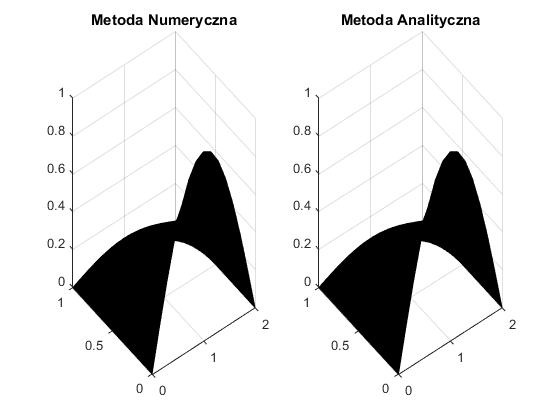
\includegraphics[width=0.78\textwidth]{Lab7/charts/btcs/5.png}
	\end{center}
\end{figure}

Czas wykonywania algorytmu $ = 0.105 s$

Dla n = 15:

\begin{figure}[!ht]
	\begin{center}
		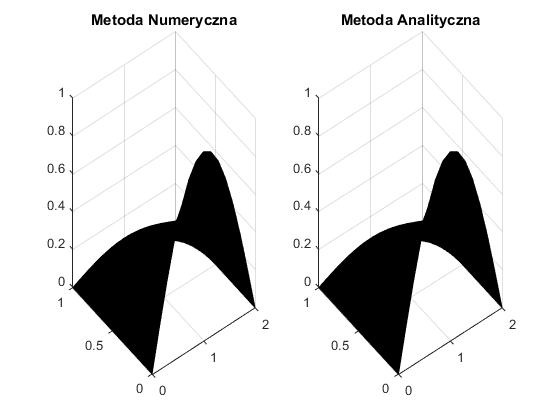
\includegraphics[width=0.78\textwidth]{Lab7/charts/btcs/15.png}
	\end{center}
\end{figure}

Czas wykonywania algorytmu $ = 0.131 s$

\newpage

Dla n = 30:

\begin{figure}[!ht]
	\begin{center}
		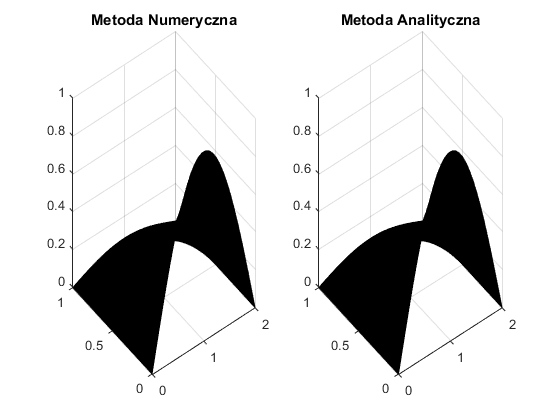
\includegraphics[width=0.78\textwidth]{Lab7/charts/btcs/30.png}
	\end{center}
\end{figure}

Czas wykonywania algorytmu $ = 0.254 s$

\subsection{Schemat Cranka-Nicolson}

$$\dfrac{\delta \psi}{\delta t} = D\dfrac{\delta^2 \psi}{\delta x^2}$$

Dla lewej strony równania zastosujemy schemat centralny na poziomie (n+$\frac{1}{2}$), natomiast dla prawej weźmiemy średnią argumentów schematów centralnych na poziomach n i n+1.

Mamy więc:

$$\dfrac{\psi^{(n+1)}_{i}-\psi^n_{i}}{\Delta t}=\dfrac{D}{2}\Bigg(\dfrac{\psi^{n+1}_{i+1}-2\psi^{n+1}_{i}+\psi^{n+1}_{i-1}}{\Delta x^2} + \dfrac{\psi^{n}_{i+1}-2\psi^{n}_{i}+\psi^{n}_{i-1}}{\Delta x^2}\Bigg) + O(\Delta t^2) + O(\Delta x^2) $$

, dalej:

$$-\alpha\psi^{n+1}_{i-1}+(2\alpha+1)\psi^{n+1}_{i}-\alpha\psi^{n+1}_{i+1}=\alpha(\psi^{n}_{i+1}-2\psi^{n}_{i}+\psi^{n}_{i-1})+\psi^{n}_{i}$$

Jest to schemat niejawny, bezwzględnie stabilny, a także jest schematem zachowawczym.

\newpage

\subsubsection{Algorytm}
\begin{Shaded}
\begin{Highlighting}[]
\FunctionTok{clc}\NormalTok{,}\FunctionTok{clear} \FunctionTok{all}\NormalTok{; }\FunctionTok{tic}
\CommentTok{%rozwiązanie analityczne}
\NormalTok{G = @(x,t) }\FunctionTok{sin}\NormalTok{(}\BaseNTok{pi}\NormalTok{.*x./}\FloatTok{2}\NormalTok{).*}\FunctionTok{exp}\NormalTok{(-(}\BaseNTok{pi}\NormalTok{.^}\FloatTok{2}\NormalTok{).*t./}\FloatTok{4}\NormalTok{);}
\CommentTok{%przedział omega}
\NormalTok{xa=}\FloatTok{0}\NormalTok{; xb=}\FloatTok{2}\NormalTok{; yc=}\FloatTok{0}\NormalTok{; yd=}\FloatTok{1}\NormalTok{;}
\CommentTok{%warunki brzegowe}
\NormalTok{ub1 = @(t) }\FloatTok{0}\NormalTok{;}
\NormalTok{ub2 = @(t) }\FloatTok{0}\NormalTok{;}
\NormalTok{up = @(x) }\FunctionTok{sin}\NormalTok{(}\BaseNTok{pi}\NormalTok{*x/}\FloatTok{2}\NormalTok{);}
\CommentTok{%siatka}
\NormalTok{n=}\FloatTok{10}\NormalTok{;}
\NormalTok{h=(xb-xa)/(n+}\FloatTok{1}\NormalTok{);}
\NormalTok{k=(yd-yc)/(n+}\FloatTok{1}\NormalTok{);}
\NormalTok{x=xa:h:xb;    }
\NormalTok{t=yc:k:yd;}
\NormalTok{D=}\FloatTok{1}\NormalTok{;}
\NormalTok{alfa = (D*k)/(}\FloatTok{2}\NormalTok{*(h^}\FloatTok{2}\NormalTok{));}
\CommentTok{%tworzenie macierzy A}
\NormalTok{A1 = -alfa*}\FunctionTok{ones}\NormalTok{(n+}\FloatTok{1}\NormalTok{,}\FloatTok{1}\NormalTok{);}
\NormalTok{A2 = (}\FloatTok{2}\NormalTok{*alfa+}\FloatTok{1}\NormalTok{)*}\FunctionTok{ones}\NormalTok{(n+}\FloatTok{2}\NormalTok{,}\FloatTok{1}\NormalTok{);}
\NormalTok{A = }\FunctionTok{diag}\NormalTok{(A1,-}\FloatTok{1}\NormalTok{) + }\FunctionTok{diag}\NormalTok{(A2) + }\FunctionTok{diag}\NormalTok{(A1,}\FloatTok{1}\NormalTok{);}
\NormalTok{A(}\FloatTok{1}\NormalTok{,}\FloatTok{1}\NormalTok{)=}\FloatTok{1}\NormalTok{; A(}\FloatTok{1}\NormalTok{,}\FloatTok{2}\NormalTok{)=}\FloatTok{0}\NormalTok{;}
\NormalTok{A(end,end)=}\FloatTok{1}\NormalTok{; A(end,end-}\FloatTok{1}\NormalTok{)=}\FloatTok{0}\NormalTok{;}
\CommentTok{%utworzenie pustej macierzy}
\NormalTok{U=}\FunctionTok{zeros}\NormalTok{(n+}\FloatTok{2}\NormalTok{,n+}\FloatTok{2}\NormalTok{); }
\CommentTok{%dodanie warunków początkowego/brzegowego}
\NormalTok{U(}\FloatTok{1}\NormalTok{,:) = up(x);}
\NormalTok{U(:,}\FloatTok{1}\NormalTok{) = ub1(t);}
\NormalTok{U(:,n+}\FloatTok{2}\NormalTok{) = ub2(t);}
\FunctionTok{psi}\NormalTok{ = }\FunctionTok{zeros}\NormalTok{(}\FloatTok{1}\NormalTok{,n+}\FloatTok{2}\NormalTok{);}
\NormalTok{licznik=}\FloatTok{0}\NormalTok{;}
\NormalTok{for }\BaseNTok{j}\NormalTok{=}\FloatTok{2}\NormalTok{:n+}\FloatTok{2}
\NormalTok{    for }\BaseNTok{i}\NormalTok{=}\FloatTok{2}\NormalTok{:n+}\FloatTok{1}
        \FunctionTok{psi}\NormalTok{(}\BaseNTok{i}\NormalTok{) = alfa*(U(}\BaseNTok{j}\NormalTok{-}\FloatTok{1}\NormalTok{,}\BaseNTok{i}\NormalTok{+}\FloatTok{1}\NormalTok{)-}\FloatTok{2}\NormalTok{*U(}\BaseNTok{j}\NormalTok{-}\FloatTok{1}\NormalTok{,}\BaseNTok{i}\NormalTok{)+U(}\BaseNTok{j}\NormalTok{-}\FloatTok{1}\NormalTok{,}\BaseNTok{i}\NormalTok{-}\FloatTok{1}\NormalTok{))+U(}\BaseNTok{j}\NormalTok{-}\FloatTok{1}\NormalTok{,}\BaseNTok{i}\NormalTok{);}
\NormalTok{    end}
\NormalTok{    F = linsolve(A,psi');}
\NormalTok{    U(}\BaseNTok{j}\NormalTok{,}\FloatTok{1}\NormalTok{:end)=F;}
\NormalTok{    licznik=licznik+}\FloatTok{1}\NormalTok{;}
\NormalTok{end}
\NormalTok{[X,T] = }\FunctionTok{meshgrid}\NormalTok{(x,t);}
\FunctionTok{subplot}\NormalTok{(}\FloatTok{1}\NormalTok{,}\FloatTok{2}\NormalTok{,}\FloatTok{1}\NormalTok{)}
\FunctionTok{surf}\NormalTok{(X,T,U)}
\FunctionTok{title}\NormalTok{(}\StringTok{'Metoda Numeryczna'}\NormalTok{)}
\FunctionTok{subplot}\NormalTok{(}\FloatTok{1}\NormalTok{,}\FloatTok{2}\NormalTok{,}\FloatTok{2}\NormalTok{)}
\FunctionTok{surf}\NormalTok{(X,T,(G(X,T)))}
\FunctionTok{title}\NormalTok{(}\StringTok{'Metoda Analityczna'}\NormalTok{)}
\NormalTok{Error=}\FunctionTok{max}\NormalTok{(}\FunctionTok{max}\NormalTok{(}\FunctionTok{abs}\NormalTok{(U-G(X,T))))}
\NormalTok{licznik; }\FunctionTok{toc}
\end{Highlighting}
\end{Shaded}
\newpage
\subsubsection{Wykresy}

Dla n = 5:

\begin{figure}[!ht]
	\begin{center}
		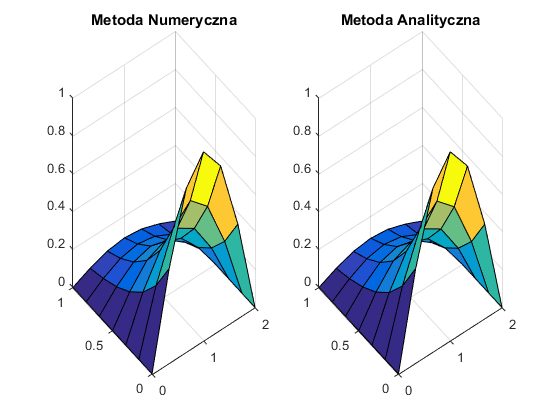
\includegraphics[width=0.78\textwidth]{Lab7/charts/cn/5.png}
	\end{center}
\end{figure}

Czas wykonywania algorytmu $ = 0.107 s$

Dla n = 15:

\begin{figure}[!ht]
	\begin{center}
		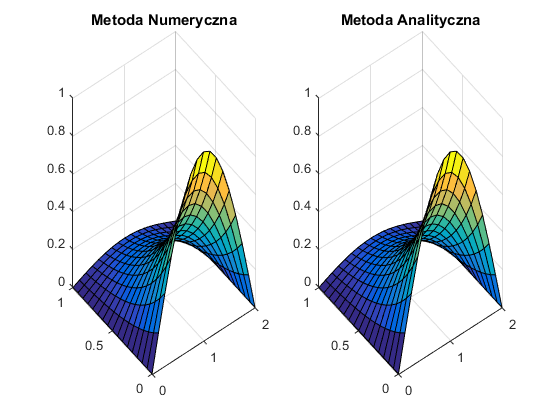
\includegraphics[width=0.78\textwidth]{Lab7/charts/cn/15.png}
	\end{center}
\end{figure}

Czas wykonywania algorytmu $ = 0.108 s$
\newpage
Dla n = 30:

\begin{figure}[!ht]
	\begin{center}
		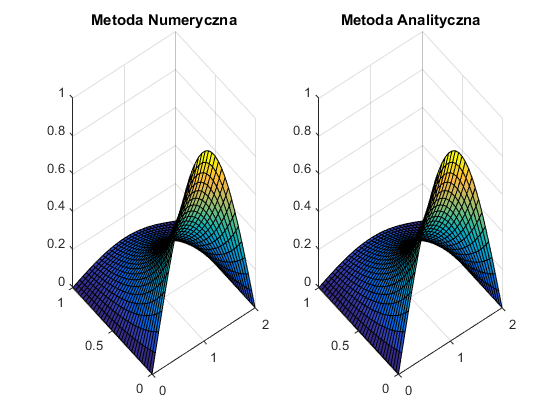
\includegraphics[width=0.78\textwidth]{Lab7/charts/cn/30.png}
	\end{center}
\end{figure}

Czas wykonywania algorytmu $ = 0.112 s$

\subsection{Schemat DuForta-Frankle}
Schemat DuForta-Frankle dla równań dyfuzyjnych postaci:

$$\dfrac{\delta \psi}{\delta t} = D\dfrac{\delta^2 \psi}{\delta x^2}$$

Dla obu stron powyższego równania stosuje się schemat centralny.

Mamy więc:

$$\dfrac{\psi^{(n+1)}_{i}-\psi^{n-1}_{i}}{2\Delta t}=D\dfrac{\psi^{n}_{i+1}- \left( \psi^{(n+1)}_{i} + \psi^{(n-1)}_{i} \right)+\psi^n_{i-1}}{\Delta x^2} + O(\Delta t^2) + O(\Delta x^2) +  O\Big(\dfrac{\Delta t}{\Delta x}\Big)^2$$

Stąd:

$$\psi^{(n+1)}_{i} \left(\dfrac{1}{2 \Delta t} + \dfrac{D}{\Delta x^2}\right)= \dfrac{D}{\Delta x^2} \left( \psi^{n}_{i+1} + \psi^{n}_{i-1} \right) - \psi^{(n-1)}_{i} \left( \dfrac{D}{\Delta x^2} + \dfrac{1}{2\Delta t} \right) $$

Jest to schemat jawny, bezwzględnie stabilny. 

Wadą tej metody jest powstawanie oscylacyjnych rozwiązań dla dużych kroków czasowych, co wpływa na jakość rozwiązania.

Jest to schemat trójpoziomowy, a więc przedstawimy dwa sposoby rozwiązania tego problemu:
\begin{itemize}
	\item skopiujemy warunek początkowy na dwa poziomy
	\item I poziom nieznany zbudujemy za pomocą schematu dwupoziomowego
\end{itemize}

\newpage
\subsubsection{Algorytm}
1)
\begin{Shaded}
\begin{Highlighting}[]
\FunctionTok{clc}\NormalTok{,}\FunctionTok{clear} \FunctionTok{all}
\FunctionTok{tic}
\CommentTok{%rozwiązanie analityczne}
\NormalTok{G = @(x,t) }\FunctionTok{sin}\NormalTok{(}\BaseNTok{pi}\NormalTok{.*x./}\FloatTok{2}\NormalTok{).*}\FunctionTok{exp}\NormalTok{(-(}\BaseNTok{pi}\NormalTok{.^}\FloatTok{2}\NormalTok{).*t./}\FloatTok{4}\NormalTok{);}
\CommentTok{%przedział omega}
\NormalTok{xa=}\FloatTok{0}\NormalTok{; xb=}\FloatTok{2}\NormalTok{; yc=}\FloatTok{0}\NormalTok{; yd=}\FloatTok{1}\NormalTok{;}
\CommentTok{%warunki brzegowe}
\NormalTok{u1 = @(x) }\FloatTok{0}\NormalTok{;}
\NormalTok{u2 = @(x) }\FloatTok{0}\NormalTok{;}
\NormalTok{u3 = @(x,t) }\FunctionTok{sin}\NormalTok{(}\BaseNTok{pi}\NormalTok{*x/}\FloatTok{2}\NormalTok{);}
\NormalTok{licznik=}\FloatTok{0}\NormalTok{;}
\CommentTok{%siatka}
\NormalTok{m=}\FloatTok{40}\NormalTok{; D=}\FloatTok{1}\NormalTok{;}
\NormalTok{deltax=(xb-xa)/(m-}\FloatTok{1}\NormalTok{);}
\NormalTok{x=[xa:deltax:xb];         }\CommentTok{%przedział przestrzenny}
\NormalTok{deltat=(deltax^}\FloatTok{2}\NormalTok{)/(}\FloatTok{10}\NormalTok{*D); }
\NormalTok{n_end=}\FunctionTok{floor}\NormalTok{(yd/deltat)+}\FloatTok{1}\NormalTok{;}
\NormalTok{t=[}\FloatTok{0}\NormalTok{:deltat:}\FloatTok{1}\NormalTok{];           }\CommentTok{%przedział czasowy}
\CommentTok{%macierz}
\FunctionTok{psi}\NormalTok{=}\FunctionTok{zeros}\NormalTok{(n_end,}\FunctionTok{length}\NormalTok{(x)); }\CommentTok{%utworzenie pustej macierzy}
\CommentTok{%dodanie warunku początkowego}
\FunctionTok{psi}\NormalTok{(}\FloatTok{1}\NormalTok{,:) = u3(x);}
\FunctionTok{psi}\NormalTok{(:,}\FloatTok{1}\NormalTok{) = u1(t);}
\FunctionTok{psi}\NormalTok{(:,m) = u2(t);}
\FunctionTok{psi}\NormalTok{(}\FloatTok{2}\NormalTok{,:) = }\FunctionTok{psi}\NormalTok{(}\FloatTok{1}\NormalTok{,:);}
\NormalTok{F = }\FunctionTok{diag}\NormalTok{(}\FunctionTok{eye}\NormalTok{(}\FloatTok{2}\NormalTok{*m-}\FloatTok{2}\NormalTok{));}
\NormalTok{A1 = }\FunctionTok{eye}\NormalTok{(m-}\FloatTok{2}\NormalTok{) .* -(D/deltax^}\FloatTok{2}\NormalTok{-}\FloatTok{1}\NormalTok{/(}\FloatTok{2}\NormalTok{*deltat));}
\NormalTok{A2 = (}\FunctionTok{eye}\NormalTok{(m-}\FloatTok{2}\NormalTok{,m) + }\FunctionTok{diag}\NormalTok{(}\FunctionTok{diag}\NormalTok{(}\FunctionTok{eye}\NormalTok{(m-}\FloatTok{2}\NormalTok{)),}\FloatTok{2}\NormalTok{)(}\FloatTok{1}\NormalTok{:m-}\FloatTok{2}\NormalTok{,:)) .* D/deltax^}\FloatTok{2}\NormalTok{;}
\NormalTok{A = [A1, A2] ./ (}\FloatTok{1}\NormalTok{/(}\FloatTok{2}\NormalTok{*deltat) + D/deltax^}\FloatTok{2}\NormalTok{);}
\NormalTok{for n=}\FloatTok{3}\NormalTok{:n_end}
\NormalTok{  F(}\FloatTok{1}\NormalTok{:m-}\FloatTok{2}\NormalTok{) = }\FunctionTok{psi}\NormalTok{(n-}\FloatTok{2}\NormalTok{,}\FloatTok{2}\NormalTok{:m-}\FloatTok{1}\NormalTok{);}
\NormalTok{  F(m-}\FloatTok{1}\NormalTok{:}\FunctionTok{length}\NormalTok{(F)) = }\FunctionTok{psi}\NormalTok{(n-}\FloatTok{1}\NormalTok{,:);}
  \FunctionTok{psi}\NormalTok{(n,}\FloatTok{2}\NormalTok{:m-}\FloatTok{1}\NormalTok{) = A * F;}
\NormalTok{  licznik = licznik+}\FloatTok{1}\NormalTok{;}
\NormalTok{end}
\NormalTok{[X,T] = }\FunctionTok{meshgrid}\NormalTok{(x,t);}
\FunctionTok{subplot}\NormalTok{(}\FloatTok{1}\NormalTok{,}\FloatTok{2}\NormalTok{,}\FloatTok{1}\NormalTok{)}
\FunctionTok{surf}\NormalTok{(X,T,}\FunctionTok{psi}\NormalTok{)}
\FunctionTok{title}\NormalTok{(}\StringTok{'Metoda Numeryczna'}\NormalTok{)}
\FunctionTok{subplot}\NormalTok{(}\FloatTok{1}\NormalTok{,}\FloatTok{2}\NormalTok{,}\FloatTok{2}\NormalTok{)}
\FunctionTok{surf}\NormalTok{(X,T,(G(X,T)))}
\FunctionTok{title}\NormalTok{(}\StringTok{'Metoda Analityczna'}\NormalTok{)}
\NormalTok{Error=}\FunctionTok{max}\NormalTok{(}\FunctionTok{max}\NormalTok{(}\FunctionTok{abs}\NormalTok{(}\FunctionTok{psi}\NormalTok{-G(X,T))));}
\NormalTok{licznik; }\FunctionTok{toc}
\end{Highlighting}
\end{Shaded}
\newpage
2)
\begin{Shaded}
\begin{Highlighting}[]
\FunctionTok{clc}\NormalTok{,}\FunctionTok{clear} \FunctionTok{all}
\FunctionTok{tic}
\CommentTok{%rozwiązanie analityczne}
\NormalTok{G = @(x,t) }\FunctionTok{sin}\NormalTok{(}\BaseNTok{pi}\NormalTok{.*x./}\FloatTok{2}\NormalTok{).*}\FunctionTok{exp}\NormalTok{(-(}\BaseNTok{pi}\NormalTok{.^}\FloatTok{2}\NormalTok{).*t./}\FloatTok{4}\NormalTok{);}
\CommentTok{%przedział omega}
\NormalTok{xa=}\FloatTok{0}\NormalTok{; xb=}\FloatTok{2}\NormalTok{; yc=}\FloatTok{0}\NormalTok{; yd=}\FloatTok{1}\NormalTok{;}
\CommentTok{%warunki brzegowe}
\NormalTok{u1 = @(x) }\FloatTok{0}\NormalTok{;}
\NormalTok{u2 = @(x) }\FloatTok{0}\NormalTok{;}
\NormalTok{u3 = @(x,t) }\FunctionTok{sin}\NormalTok{(}\BaseNTok{pi}\NormalTok{*x/}\FloatTok{2}\NormalTok{);}
\NormalTok{licznik=}\FloatTok{0}\NormalTok{;}
\CommentTok{%siatka}
\NormalTok{m=}\FloatTok{40}\NormalTok{; D=}\FloatTok{1}\NormalTok{;}
\NormalTok{deltax=(xb-xa)/(m-}\FloatTok{1}\NormalTok{);}
\NormalTok{x=[xa:deltax:xb];         }\CommentTok{%przedział przestrzenny}
\NormalTok{deltat=(deltax^}\FloatTok{2}\NormalTok{)/(}\FloatTok{10}\NormalTok{*D); }
\NormalTok{n_end=}\FunctionTok{floor}\NormalTok{(yd/deltat)+}\FloatTok{1}\NormalTok{;}
\NormalTok{t=[}\FloatTok{0}\NormalTok{:deltat:}\FloatTok{1}\NormalTok{];           }\CommentTok{%przedział czasowy}
\CommentTok{%macierz}
\FunctionTok{psi}\NormalTok{=}\FunctionTok{zeros}\NormalTok{(n_end,}\FunctionTok{length}\NormalTok{(x)); }\CommentTok{%utworzenie pustej macierzy}
\CommentTok{%dodanie warunku początkowego}
\FunctionTok{psi}\NormalTok{(}\FloatTok{1}\NormalTok{,:) = u3(x);}
\FunctionTok{psi}\NormalTok{(:,}\FloatTok{1}\NormalTok{) = u1(t);}
\FunctionTok{psi}\NormalTok{(:,m) = u2(t);}
\CommentTok{% Pierwszy poziom za pomocą schematu dwupoziomowego}
\NormalTok{A_2 = (}\FloatTok{2}\NormalTok{+(deltax^}\FloatTok{2}\NormalTok{)/(deltat))*}\FunctionTok{diag}\NormalTok{(}\FunctionTok{eye}\NormalTok{(m-}\FloatTok{2}\NormalTok{));}
\NormalTok{B_2 = }\FunctionTok{diag}\NormalTok{(A_2) + -}\FloatTok{1}\NormalTok{*}\FunctionTok{diag}\NormalTok{(}\FunctionTok{diag}\NormalTok{(}\FunctionTok{eye}\NormalTok{(m-}\FloatTok{3}\NormalTok{)),-}\FloatTok{1}\NormalTok{) + -}\FloatTok{1}\NormalTok{*}\FunctionTok{diag}\NormalTok{(}\FunctionTok{diag}\NormalTok{(}\FunctionTok{eye}\NormalTok{(m-}\FloatTok{3}\NormalTok{)),}\FloatTok{1}\NormalTok{);}
\NormalTok{F = }\FunctionTok{diag}\NormalTok{(}\FunctionTok{eye}\NormalTok{(m-}\FloatTok{2}\NormalTok{)) * deltax^}\FloatTok{2}\NormalTok{/deltat .* }\FunctionTok{psi}\NormalTok{(}\FloatTok{1}\NormalTok{,}\FloatTok{2}\NormalTok{:m-}\FloatTok{1}\NormalTok{)';}
\NormalTok{F(}\FloatTok{1}\NormalTok{) = F(}\FloatTok{1}\NormalTok{) + }\FunctionTok{psi}\NormalTok{(}\FloatTok{2}\NormalTok{,}\FloatTok{1}\NormalTok{);}
\NormalTok{F(}\FunctionTok{length}\NormalTok{(F)) = F(}\FunctionTok{length}\NormalTok{(F)) + }\FunctionTok{psi}\NormalTok{(}\FloatTok{2}\NormalTok{, m);  }
\FunctionTok{psi}\NormalTok{(}\FloatTok{2}\NormalTok{,}\FloatTok{2}\NormalTok{:m-}\FloatTok{1}\NormalTok{) = linsolve(B_2,F);}
\CommentTok{% Pozostałe poziomy}
\NormalTok{F = }\FunctionTok{diag}\NormalTok{(}\FunctionTok{eye}\NormalTok{(}\FloatTok{2}\NormalTok{*m-}\FloatTok{2}\NormalTok{));}
\NormalTok{A1 = }\FunctionTok{eye}\NormalTok{(m-}\FloatTok{2}\NormalTok{) .* -(D/deltax^}\FloatTok{2}\NormalTok{-}\FloatTok{1}\NormalTok{/(}\FloatTok{2}\NormalTok{*deltat));}
\NormalTok{A2 = (}\FunctionTok{eye}\NormalTok{(m-}\FloatTok{2}\NormalTok{,m) + }\FunctionTok{diag}\NormalTok{(}\FunctionTok{diag}\NormalTok{(}\FunctionTok{eye}\NormalTok{(m-}\FloatTok{2}\NormalTok{)),}\FloatTok{2}\NormalTok{)(}\FloatTok{1}\NormalTok{:m-}\FloatTok{2}\NormalTok{,:)) .* D/deltax^}\FloatTok{2}\NormalTok{;}
\NormalTok{A = [A1, A2] ./ (}\FloatTok{1}\NormalTok{/(}\FloatTok{2}\NormalTok{*deltat) + D/deltax^}\FloatTok{2}\NormalTok{);}
\NormalTok{for n=}\FloatTok{3}\NormalTok{:n_end}
\NormalTok{  F(}\FloatTok{1}\NormalTok{:m-}\FloatTok{2}\NormalTok{) = }\FunctionTok{psi}\NormalTok{(n-}\FloatTok{2}\NormalTok{,}\FloatTok{2}\NormalTok{:m-}\FloatTok{1}\NormalTok{);}
\NormalTok{  F(m-}\FloatTok{1}\NormalTok{:}\FunctionTok{length}\NormalTok{(F)) = }\FunctionTok{psi}\NormalTok{(n-}\FloatTok{1}\NormalTok{,:);}
  \FunctionTok{psi}\NormalTok{(n,}\FloatTok{2}\NormalTok{:m-}\FloatTok{1}\NormalTok{) = A * F;}
\NormalTok{  licznik = licznik+}\FloatTok{1}\NormalTok{;}
\NormalTok{end}
\NormalTok{[X,T] = }\FunctionTok{meshgrid}\NormalTok{(x,t);}
\FunctionTok{subplot}\NormalTok{(}\FloatTok{1}\NormalTok{,}\FloatTok{2}\NormalTok{,}\FloatTok{1}\NormalTok{)}
\FunctionTok{surf}\NormalTok{(X,T,}\FunctionTok{psi}\NormalTok{)}
\FunctionTok{title}\NormalTok{(}\StringTok{'Metoda Numeryczna'}\NormalTok{)}
\FunctionTok{subplot}\NormalTok{(}\FloatTok{1}\NormalTok{,}\FloatTok{2}\NormalTok{,}\FloatTok{2}\NormalTok{)}
\FunctionTok{surf}\NormalTok{(X,T,(G(X,T)))}
\FunctionTok{title}\NormalTok{(}\StringTok{'Metoda Analityczna'}\NormalTok{)}
\NormalTok{Error=}\FunctionTok{max}\NormalTok{(}\FunctionTok{max}\NormalTok{(}\FunctionTok{abs}\NormalTok{(}\FunctionTok{psi}\NormalTok{-G(X,T))));}
\NormalTok{licznik; }\FunctionTok{toc}
\end{Highlighting}
\end{Shaded}
\newpage
\subsubsection{Wykresy}
1)

Dla n = 5:

\begin{figure}[!ht]
	\begin{center}
		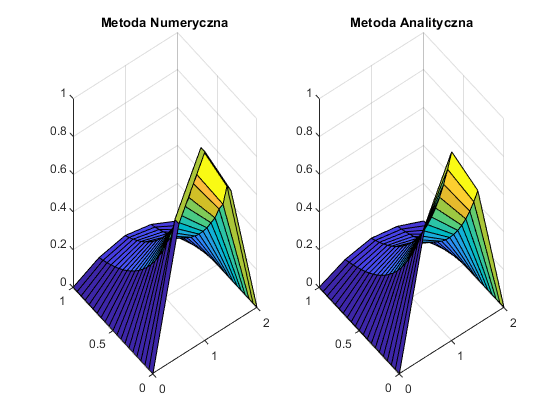
\includegraphics[width=0.78\textwidth]{Lab7/charts/df/5.png}
	\end{center}
\end{figure}

Czas wykonywania algorytmu $ = 0.096 s$

%\newpage

Dla n = 15:

\begin{figure}[!ht]
	\begin{center}
		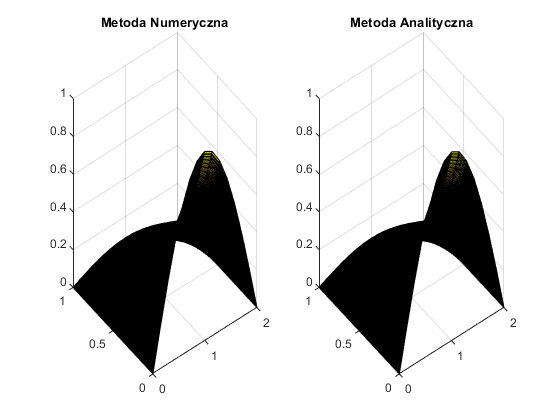
\includegraphics[width=0.78\textwidth]{Lab7/charts/df/15.png}
	\end{center}
\end{figure}

Czas wykonywania algorytmu $ = 0.099 s$
\newpage
Dla n = 30:

\begin{figure}[!ht]
	\begin{center}
		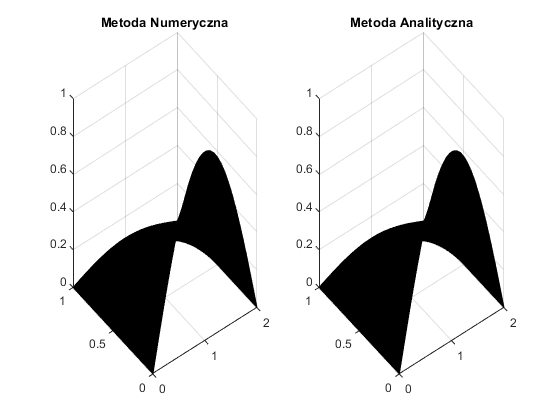
\includegraphics[width=0.78\textwidth]{Lab7/charts/df/30.png}
	\end{center}
\end{figure}

Czas wykonywania algorytmu $ = 0.113 s$

Dla n = 30 oraz $\Delta t = 0.047562$:

\begin{figure}[!ht]
	\begin{center}
		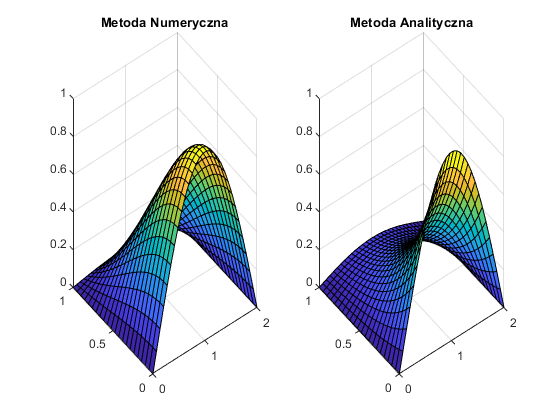
\includegraphics[width=0.78\textwidth]{Lab7/charts/df/30_k.png}
	\end{center}
\end{figure}

Czas wykonywania algorytmu $ = 0.095 s$

\FloatBarrier
\newpage
2)\\

Dla n = 5:

\begin{figure}[!ht]
	\begin{center}
		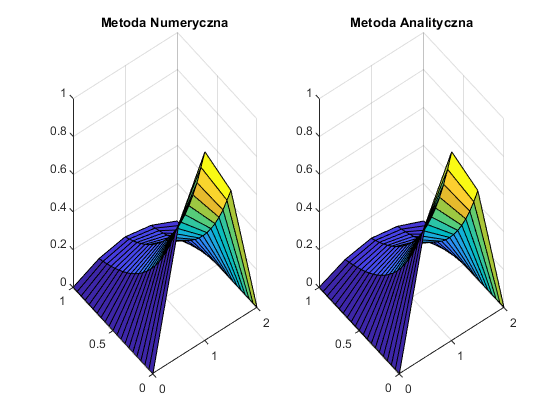
\includegraphics[width=0.78\textwidth]{Lab7/charts/df/5_2.png}
	\end{center}
\end{figure}

Czas wykonywania algorytmu $ = 0.101 s$

Dla n = 15:

\begin{figure}[!ht]
	\begin{center}
		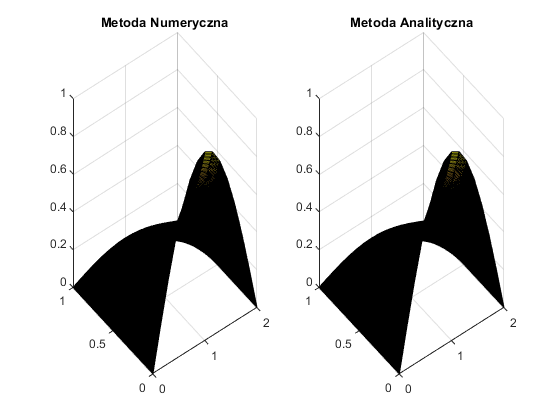
\includegraphics[width=0.78\textwidth]{Lab7/charts/df/15_2.png}
	\end{center}
\end{figure}

Czas wykonywania algorytmu $ = 0.103 s$
\newpage
Dla n = 30:

\begin{figure}[!ht]
	\begin{center}
		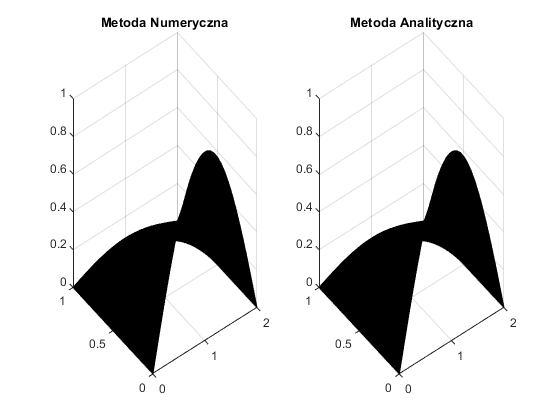
\includegraphics[width=0.78\textwidth]{Lab7/charts/df/30_2.png}
	\end{center}
\end{figure}

Czas wykonywania algorytmu $ = 0.117 s$

Dla n = 30 oraz $\Delta t = 0.047562$:

\begin{figure}[!ht]
	\begin{center}
		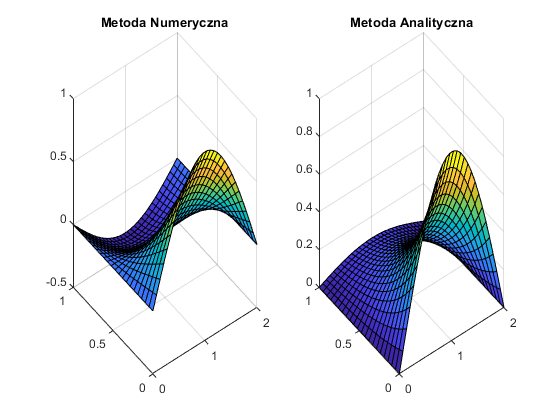
\includegraphics[width=0.78\textwidth]{Lab7/charts/df/30_2_k.png}
	\end{center}
\end{figure}

Czas wykonywania algorytmu $ = 0.098 s$

\newpage
\subsection{Schemat Richtmyera-Morton}

Niejawna metoda trójpoziomowa, charakteryzująca się znakomitą dokładnością.

$$\dfrac{\delta \psi}{\delta t} = D\dfrac{\delta^2 \psi}{\delta x^2}$$

, mamy:

$$(1+\Theta)\dfrac{\psi^{n+1}_{i}-\psi^n_{i}}{\Delta t}-\Theta\dfrac{\psi^{n}_{i}-\psi^{n-1}_{i}}{\Delta t} = D \dfrac{\psi^{n+1}_{i+1}-2\psi^{n+1}_{i}+\psi^{n+1}_{i-1}}{\Delta x^2} + O(\Delta t^2) + O(\Delta x^2) $$

, oznaczmy:

$$\dfrac{D\Delta t}{\Delta x^2} = \alpha$$

, zwiększamy dokładność do  $O(\Delta t^2) + O(\Delta x^4)$ , niech:

$$\Theta = \frac{1}{2} - \dfrac{\Delta x^2}{12D\Delta t}$$

, po trywialnych przekształceniach:

$$-\alpha\psi^{n+1}_{i-1}+(1+\Theta + 2\alpha)\psi^{n+1}_{i}-\alpha\psi^{n+1}_{i+1}=(1+2\Theta)\psi^{n}_{i} - \Theta\psi^{n-1}_{i}$$

$$A\psi^{n+1}=\widetilde{\psi}^{n}+\widetilde{\psi}^{n-1}$$

\newpage

\subsubsection{Algorytm}
1)
\begin{Shaded}
\begin{Highlighting}[]
\FunctionTok{clc}\NormalTok{,}\FunctionTok{clear} \FunctionTok{all}\NormalTok{; }\FunctionTok{tic}
\CommentTok{%rozwiązanie analityczne}
\NormalTok{G = @(x,t) }\FunctionTok{sin}\NormalTok{(}\BaseNTok{pi}\NormalTok{.*x./}\FloatTok{2}\NormalTok{).*}\FunctionTok{exp}\NormalTok{(-(}\BaseNTok{pi}\NormalTok{.^}\FloatTok{2}\NormalTok{).*t./}\FloatTok{4}\NormalTok{);}
\CommentTok{%przedział omega}
\NormalTok{xa=}\FloatTok{0}\NormalTok{; xb=}\FloatTok{2}\NormalTok{; yc=}\FloatTok{0}\NormalTok{; yd=}\FloatTok{1}\NormalTok{;}
\CommentTok{%warunki brzegowe}
\NormalTok{u1 = @(x) }\FloatTok{0}\NormalTok{;}
\NormalTok{u2 = @(x) }\FloatTok{0}\NormalTok{;}
\NormalTok{u3 = @(x,t) }\FunctionTok{sin}\NormalTok{(}\BaseNTok{pi}\NormalTok{*x/}\FloatTok{2}\NormalTok{);}
\NormalTok{licznik=}\FloatTok{0}\NormalTok{;}
\CommentTok{%siatka}
\NormalTok{m=}\FloatTok{50}\NormalTok{; D=}\FloatTok{1}\NormalTok{;}
\NormalTok{deltax=(xb-xa)/(m-}\FloatTok{1}\NormalTok{);}
\NormalTok{x=[xa:deltax:xb];         }\CommentTok{%przedział przestrzenny}
\NormalTok{deltat=(deltax^}\FloatTok{2}\NormalTok{)/D; n_end=}\FunctionTok{floor}\NormalTok{(yd/deltat)+}\FloatTok{1}\NormalTok{;}
\NormalTok{t=[}\FloatTok{0}\NormalTok{:deltat:}\FloatTok{1}\NormalTok{];           }\CommentTok{%przedział czasowy}
\NormalTok{theta = }\FloatTok{1}\NormalTok{/}\FloatTok{2}\NormalTok{ - deltax^}\FloatTok{2}\NormalTok{ / (}\FloatTok{12}\NormalTok{ * D * deltat);}
\NormalTok{alfa = D * deltat / deltax^}\FloatTok{2}\NormalTok{;}
\CommentTok{%macierz}
\FunctionTok{psi}\NormalTok{=}\FunctionTok{zeros}\NormalTok{(n_end,}\FunctionTok{length}\NormalTok{(x)); }\CommentTok{%utworzenie pustej macierzy}
\CommentTok{%dodanie warunku początkowego}
\FunctionTok{psi}\NormalTok{(}\FloatTok{1}\NormalTok{,:) = u3(x);}
\FunctionTok{psi}\NormalTok{(:,}\FloatTok{1}\NormalTok{) = u1(t);}
\FunctionTok{psi}\NormalTok{(:,m) = u2(t);}
\CommentTok{% Skopiowanie pierwszego kroku }
\FunctionTok{psi}\NormalTok{(}\FloatTok{2}\NormalTok{,:) = }\FunctionTok{psi}\NormalTok{(}\FloatTok{1}\NormalTok{,:);}
\NormalTok{F = }\FunctionTok{diag}\NormalTok{(}\FunctionTok{eye}\NormalTok{(m-}\FloatTok{2}\NormalTok{));}
\NormalTok{A1 = }\FunctionTok{eye}\NormalTok{(m-}\FloatTok{2}\NormalTok{) .* (}\FloatTok{2}\NormalTok{*alfa + }\FloatTok{1}\NormalTok{ + theta);}
\NormalTok{A2 = }\FunctionTok{diag}\NormalTok{(}\FunctionTok{eye}\NormalTok{(m-}\FloatTok{3}\NormalTok{)) * -alfa;}
\NormalTok{A = A1 + }\FunctionTok{diag}\NormalTok{(A2,-}\FloatTok{1}\NormalTok{) + }\FunctionTok{diag}\NormalTok{(A2, }\FloatTok{1}\NormalTok{);}
\NormalTok{for n=}\FloatTok{3}\NormalTok{:n_end}
\NormalTok{  F = (}\FloatTok{1}\NormalTok{+}\FloatTok{2}\NormalTok{*theta) * }\FunctionTok{psi}\NormalTok{(n-}\FloatTok{1}\NormalTok{,}\FloatTok{2}\NormalTok{:m-}\FloatTok{1}\NormalTok{) - theta * }\FunctionTok{psi}\NormalTok{(n-}\FloatTok{2}\NormalTok{, }\FloatTok{2}\NormalTok{:m-}\FloatTok{1}\NormalTok{);}
\NormalTok{  F(}\FloatTok{1}\NormalTok{) = F(}\FloatTok{1}\NormalTok{) + alfa * }\FunctionTok{psi}\NormalTok{(n, }\FloatTok{1}\NormalTok{);}
\NormalTok{  F(m-}\FloatTok{2}\NormalTok{) = F(m-}\FloatTok{2}\NormalTok{) + alfa * }\FunctionTok{psi}\NormalTok{(n, m);}
  \FunctionTok{psi}\NormalTok{(n,}\FloatTok{2}\NormalTok{:m-}\FloatTok{1}\NormalTok{) = linsolve(A,F');}
\NormalTok{  licznik = licznik+}\FloatTok{1}\NormalTok{;}
\NormalTok{end}
\NormalTok{[X,T] = }\FunctionTok{meshgrid}\NormalTok{(x,t);}
\FunctionTok{subplot}\NormalTok{(}\FloatTok{1}\NormalTok{,}\FloatTok{2}\NormalTok{,}\FloatTok{1}\NormalTok{)}
\FunctionTok{surf}\NormalTok{(X,T,}\FunctionTok{psi}\NormalTok{)}
\FunctionTok{title}\NormalTok{(}\StringTok{'Metoda Numeryczna'}\NormalTok{)}
\FunctionTok{subplot}\NormalTok{(}\FloatTok{1}\NormalTok{,}\FloatTok{2}\NormalTok{,}\FloatTok{2}\NormalTok{)}
\FunctionTok{surf}\NormalTok{(X,T,(G(X,T)))}
\FunctionTok{title}\NormalTok{(}\StringTok{'Metoda Analityczna'}\NormalTok{)}
\NormalTok{Error=}\FunctionTok{max}\NormalTok{(}\FunctionTok{max}\NormalTok{(}\FunctionTok{abs}\NormalTok{(}\FunctionTok{psi}\NormalTok{-G(X,T))));}
\NormalTok{licznik; }\FunctionTok{toc}
\end{Highlighting}
\end{Shaded}
\newpage
2)
\begin{Shaded}
\begin{Highlighting}[]
\FunctionTok{clc}\NormalTok{, }\FunctionTok{clear} \FunctionTok{all}\NormalTok{; }\FunctionTok{tic}
\CommentTok{%rozwiązanie analityczne}
\NormalTok{G = @(x,t) }\FunctionTok{sin}\NormalTok{(}\BaseNTok{pi}\NormalTok{.*x./}\FloatTok{2}\NormalTok{).*}\FunctionTok{exp}\NormalTok{(-(}\BaseNTok{pi}\NormalTok{.^}\FloatTok{2}\NormalTok{).*t./}\FloatTok{4}\NormalTok{);}
\CommentTok{%przedział omega}
\NormalTok{xa=}\FloatTok{0}\NormalTok{; xb=}\FloatTok{2}\NormalTok{; yc=}\FloatTok{0}\NormalTok{; yd=}\FloatTok{1}\NormalTok{;}
\CommentTok{%warunki brzegowe}
\NormalTok{u1 = @(x) }\FloatTok{0}\NormalTok{; u2 = @(x) }\FloatTok{0}\NormalTok{; u3 = @(x,t) }\FunctionTok{sin}\NormalTok{(}\BaseNTok{pi}\NormalTok{*x/}\FloatTok{2}\NormalTok{);}
\NormalTok{licznik=}\FloatTok{0}\NormalTok{;}
\CommentTok{%siatka}
\NormalTok{m=}\FloatTok{50}\NormalTok{; D=}\FloatTok{1}\NormalTok{; deltax=(xb-xa)/(m-}\FloatTok{1}\NormalTok{);}
\NormalTok{x=[xa:deltax:xb];         }\CommentTok{%przedział przestrzenny}
\NormalTok{deltat=(deltax^}\FloatTok{2}\NormalTok{)/D; }
\NormalTok{n_end=}\FunctionTok{floor}\NormalTok{(yd/deltat)+}\FloatTok{1}\NormalTok{;}
\NormalTok{t=[}\FloatTok{0}\NormalTok{:deltat:}\FloatTok{1}\NormalTok{];           }\CommentTok{%przedział czasowy}
\NormalTok{theta = }\FloatTok{1}\NormalTok{/}\FloatTok{2}\NormalTok{ - deltax^}\FloatTok{2}\NormalTok{ / (}\FloatTok{12}\NormalTok{ * D * deltat);}
\NormalTok{alfa = D * deltat / deltax^}\FloatTok{2}\NormalTok{;}
\CommentTok{%macierz}
\FunctionTok{psi}\NormalTok{=}\FunctionTok{zeros}\NormalTok{(n_end,}\FunctionTok{length}\NormalTok{(x)); }\CommentTok{%utworzenie pustej macierzy}
\CommentTok{%dodanie warunku początkowego}
\FunctionTok{psi}\NormalTok{(}\FloatTok{1}\NormalTok{,:) = u3(x);}
\FunctionTok{psi}\NormalTok{(:,}\FloatTok{1}\NormalTok{) = u1(t);}
\FunctionTok{psi}\NormalTok{(:,m) = u2(t);}
\NormalTok{A1 = }\FunctionTok{eye}\NormalTok{(m-}\FloatTok{2}\NormalTok{) .* (}\FloatTok{2}\NormalTok{*alfa + }\FloatTok{1}\NormalTok{ + theta);}
\NormalTok{A2 = }\FunctionTok{diag}\NormalTok{(}\FunctionTok{eye}\NormalTok{(m-}\FloatTok{3}\NormalTok{)) * -alfa;}
\NormalTok{A = A1 + }\FunctionTok{diag}\NormalTok{(A2,-}\FloatTok{1}\NormalTok{) + }\FunctionTok{diag}\NormalTok{(A2, }\FloatTok{1}\NormalTok{);}
\CommentTok{% Pierwszy poziom za pomocą schematu dwupoziomowego}
\NormalTok{A_2 = (}\FloatTok{2}\NormalTok{+(deltax^}\FloatTok{2}\NormalTok{)/(deltat))*}\FunctionTok{diag}\NormalTok{(}\FunctionTok{eye}\NormalTok{(m-}\FloatTok{2}\NormalTok{));}
\NormalTok{B_2 = }\FunctionTok{diag}\NormalTok{(A_2) + -}\FloatTok{1}\NormalTok{*}\FunctionTok{diag}\NormalTok{(}\FunctionTok{diag}\NormalTok{(}\FunctionTok{eye}\NormalTok{(m-}\FloatTok{3}\NormalTok{)),-}\FloatTok{1}\NormalTok{) + -}\FloatTok{1}\NormalTok{*}\FunctionTok{diag}\NormalTok{(}\FunctionTok{diag}\NormalTok{(}\FunctionTok{eye}\NormalTok{(m-}\FloatTok{3}\NormalTok{)),}\FloatTok{1}\NormalTok{);}
\NormalTok{F = }\FunctionTok{diag}\NormalTok{(}\FunctionTok{eye}\NormalTok{(m-}\FloatTok{2}\NormalTok{)) * deltax^}\FloatTok{2}\NormalTok{/deltat .* }\FunctionTok{psi}\NormalTok{(}\FloatTok{1}\NormalTok{,}\FloatTok{2}\NormalTok{:m-}\FloatTok{1}\NormalTok{)';}
\NormalTok{F(}\FloatTok{1}\NormalTok{) = F(}\FloatTok{1}\NormalTok{) + }\FunctionTok{psi}\NormalTok{(}\FloatTok{2}\NormalTok{,}\FloatTok{1}\NormalTok{); F(}\FunctionTok{length}\NormalTok{(F)) = F(}\FunctionTok{length}\NormalTok{(F)) + }\FunctionTok{psi}\NormalTok{(}\FloatTok{2}\NormalTok{, m);  }
\FunctionTok{psi}\NormalTok{(}\FloatTok{2}\NormalTok{,}\FloatTok{2}\NormalTok{:m-}\FloatTok{1}\NormalTok{) = linsolve(B_2,F);}
\CommentTok{% Pozostałe poziomy}
\NormalTok{for n=}\FloatTok{3}\NormalTok{:n_end}
\NormalTok{  F = (}\FloatTok{1}\NormalTok{+}\FloatTok{2}\NormalTok{*theta) * }\FunctionTok{psi}\NormalTok{(n-}\FloatTok{1}\NormalTok{,}\FloatTok{2}\NormalTok{:m-}\FloatTok{1}\NormalTok{) - theta * }\FunctionTok{psi}\NormalTok{(n-}\FloatTok{2}\NormalTok{, }\FloatTok{2}\NormalTok{:m-}\FloatTok{1}\NormalTok{);}
\NormalTok{  F(}\FloatTok{1}\NormalTok{) = F(}\FloatTok{1}\NormalTok{) + alfa * }\FunctionTok{psi}\NormalTok{(n, }\FloatTok{1}\NormalTok{);}
\NormalTok{  F(m-}\FloatTok{2}\NormalTok{) = F(m-}\FloatTok{2}\NormalTok{) + alfa * }\FunctionTok{psi}\NormalTok{(n, m);}
  \FunctionTok{psi}\NormalTok{(n,}\FloatTok{2}\NormalTok{:m-}\FloatTok{1}\NormalTok{) = linsolve(A,F');}
\NormalTok{  licznik = licznik+}\FloatTok{1}\NormalTok{;}
\NormalTok{end}
\NormalTok{[X,T] = }\FunctionTok{meshgrid}\NormalTok{(x,t);}
\FunctionTok{subplot}\NormalTok{(}\FloatTok{1}\NormalTok{,}\FloatTok{2}\NormalTok{,}\FloatTok{1}\NormalTok{)}
\FunctionTok{surf}\NormalTok{(X,T,}\FunctionTok{psi}\NormalTok{)}
\FunctionTok{title}\NormalTok{(}\StringTok{'Metoda Numeryczna'}\NormalTok{)}
\FunctionTok{subplot}\NormalTok{(}\FloatTok{1}\NormalTok{,}\FloatTok{2}\NormalTok{,}\FloatTok{2}\NormalTok{)}
\FunctionTok{surf}\NormalTok{(X,T,(G(X,T)))}
\FunctionTok{title}\NormalTok{(}\StringTok{'Metoda Analityczna'}\NormalTok{)}
\NormalTok{Error=}\FunctionTok{max}\NormalTok{(}\FunctionTok{max}\NormalTok{(}\FunctionTok{abs}\NormalTok{(}\FunctionTok{psi}\NormalTok{-G(X,T))));}
\NormalTok{licznik; }\FunctionTok{toc}
\end{Highlighting}
\end{Shaded}
\newpage
\subsubsection{Wykresy}
1)

Dla n = 5:

\begin{figure}[!ht]
	\begin{center}
		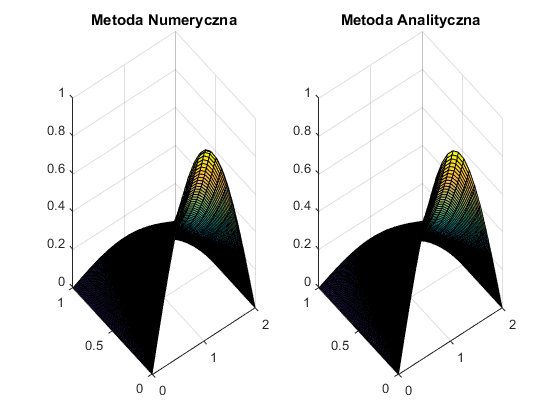
\includegraphics[width=0.8\textwidth]{Lab7/charts/rm/5.png}
	\end{center}
\end{figure}

Czas wykonywania algorytmu $ = 0.097 s$

Dla n = 15:

\begin{figure}[!ht]
	\begin{center}
		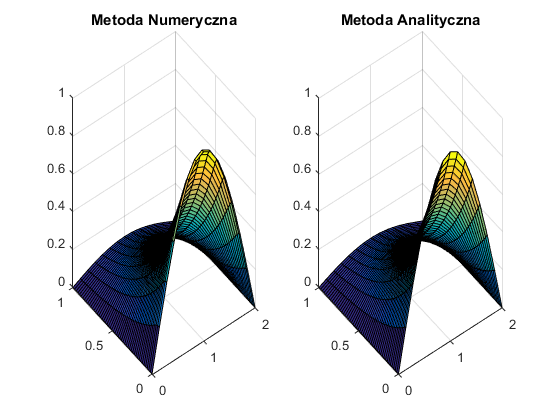
\includegraphics[width=0.8\textwidth]{Lab7/charts/rm/15.png}
	\end{center}
\end{figure}

Czas wykonywania algorytmu $ = 0.103 s$

\newpage

Dla n = 30:

\begin{figure}[!ht]
	\begin{center}
		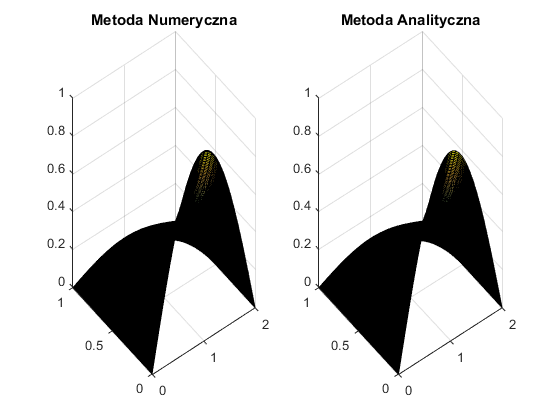
\includegraphics[width=0.8\textwidth]{Lab7/charts/rm/30.png}
	\end{center}
\end{figure}

Czas wykonywania algorytmu $ = 0.105 s$

2)

Dla n = 20:

\begin{figure}[!ht]
	\begin{center}
		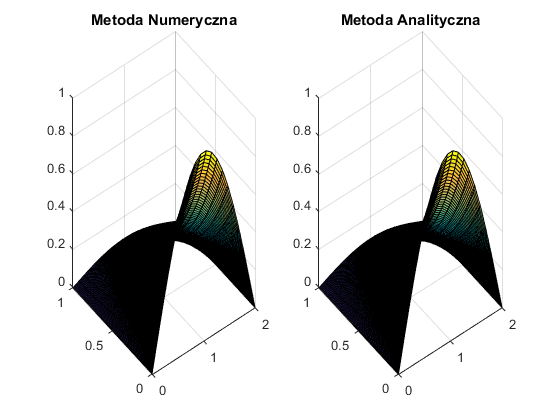
\includegraphics[width=0.8\textwidth]{Lab7/charts/rmb/20.png}
	\end{center}
\end{figure}

Czas wykonywania algorytmu $ = 0.103s$

\newpage

Dla n = 50:

\begin{figure}[!ht]
	\begin{center}
		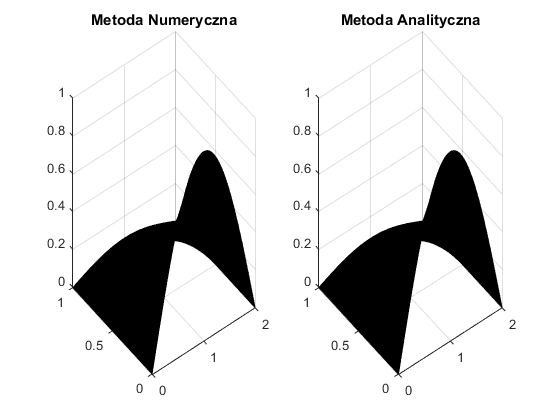
\includegraphics[width=0.8\textwidth]{Lab7/charts/rmb/50.png}
	\end{center}
\end{figure}

Czas wykonywania algorytmu $ = 0.131s$

Dla n = 100:

\begin{figure}[!ht]
	\begin{center}
		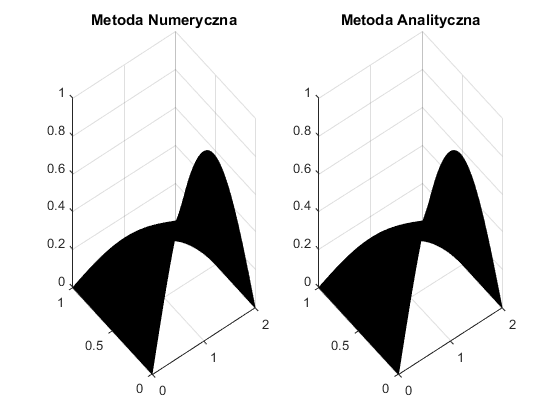
\includegraphics[width=0.8\textwidth]{Lab7/charts/rmb/100.png}
	\end{center}
\end{figure}

Czas wykonywania algorytmu $ = 0.433s$
